% Options for packages loaded elsewhere
\PassOptionsToPackage{unicode}{hyperref}
\PassOptionsToPackage{hyphens}{url}
%
\documentclass[
  man]{apa6}
\usepackage{amsmath,amssymb}
\usepackage{iftex}
\ifPDFTeX
  \usepackage[T1]{fontenc}
  \usepackage[utf8]{inputenc}
  \usepackage{textcomp} % provide euro and other symbols
\else % if luatex or xetex
  \usepackage{unicode-math} % this also loads fontspec
  \defaultfontfeatures{Scale=MatchLowercase}
  \defaultfontfeatures[\rmfamily]{Ligatures=TeX,Scale=1}
\fi
\usepackage{lmodern}
\ifPDFTeX\else
  % xetex/luatex font selection
\fi
% Use upquote if available, for straight quotes in verbatim environments
\IfFileExists{upquote.sty}{\usepackage{upquote}}{}
\IfFileExists{microtype.sty}{% use microtype if available
  \usepackage[]{microtype}
  \UseMicrotypeSet[protrusion]{basicmath} % disable protrusion for tt fonts
}{}
\makeatletter
\@ifundefined{KOMAClassName}{% if non-KOMA class
  \IfFileExists{parskip.sty}{%
    \usepackage{parskip}
  }{% else
    \setlength{\parindent}{0pt}
    \setlength{\parskip}{6pt plus 2pt minus 1pt}}
}{% if KOMA class
  \KOMAoptions{parskip=half}}
\makeatother
\usepackage{xcolor}
\usepackage{longtable,booktabs,array}
\usepackage{calc} % for calculating minipage widths
% Correct order of tables after \paragraph or \subparagraph
\usepackage{etoolbox}
\makeatletter
\patchcmd\longtable{\par}{\if@noskipsec\mbox{}\fi\par}{}{}
\makeatother
% Allow footnotes in longtable head/foot
\IfFileExists{footnotehyper.sty}{\usepackage{footnotehyper}}{\usepackage{footnote}}
\makesavenoteenv{longtable}
\usepackage{graphicx}
\makeatletter
\def\maxwidth{\ifdim\Gin@nat@width>\linewidth\linewidth\else\Gin@nat@width\fi}
\def\maxheight{\ifdim\Gin@nat@height>\textheight\textheight\else\Gin@nat@height\fi}
\makeatother
% Scale images if necessary, so that they will not overflow the page
% margins by default, and it is still possible to overwrite the defaults
% using explicit options in \includegraphics[width, height, ...]{}
\setkeys{Gin}{width=\maxwidth,height=\maxheight,keepaspectratio}
% Set default figure placement to htbp
\makeatletter
\def\fps@figure{htbp}
\makeatother
\setlength{\emergencystretch}{3em} % prevent overfull lines
\providecommand{\tightlist}{%
  \setlength{\itemsep}{0pt}\setlength{\parskip}{0pt}}
\setcounter{secnumdepth}{-\maxdimen} % remove section numbering
% Make \paragraph and \subparagraph free-standing
\ifx\paragraph\undefined\else
  \let\oldparagraph\paragraph
  \renewcommand{\paragraph}[1]{\oldparagraph{#1}\mbox{}}
\fi
\ifx\subparagraph\undefined\else
  \let\oldsubparagraph\subparagraph
  \renewcommand{\subparagraph}[1]{\oldsubparagraph{#1}\mbox{}}
\fi
\newlength{\cslhangindent}
\setlength{\cslhangindent}{1.5em}
\newlength{\csllabelwidth}
\setlength{\csllabelwidth}{3em}
\newlength{\cslentryspacingunit} % times entry-spacing
\setlength{\cslentryspacingunit}{\parskip}
\newenvironment{CSLReferences}[2] % #1 hanging-ident, #2 entry spacing
 {% don't indent paragraphs
  \setlength{\parindent}{0pt}
  % turn on hanging indent if param 1 is 1
  \ifodd #1
  \let\oldpar\par
  \def\par{\hangindent=\cslhangindent\oldpar}
  \fi
  % set entry spacing
  \setlength{\parskip}{#2\cslentryspacingunit}
 }%
 {}
\usepackage{calc}
\newcommand{\CSLBlock}[1]{#1\hfill\break}
\newcommand{\CSLLeftMargin}[1]{\parbox[t]{\csllabelwidth}{#1}}
\newcommand{\CSLRightInline}[1]{\parbox[t]{\linewidth - \csllabelwidth}{#1}\break}
\newcommand{\CSLIndent}[1]{\hspace{\cslhangindent}#1}
\ifLuaTeX
\usepackage[bidi=basic]{babel}
\else
\usepackage[bidi=default]{babel}
\fi
\babelprovide[main,import]{english}
% get rid of language-specific shorthands (see #6817):
\let\LanguageShortHands\languageshorthands
\def\languageshorthands#1{}
% Manuscript styling
\usepackage{upgreek}
\captionsetup{font=singlespacing,justification=justified}

% Table formatting
\usepackage{longtable}
\usepackage{lscape}
% \usepackage[counterclockwise]{rotating}   % Landscape page setup for large tables
\usepackage{multirow}		% Table styling
\usepackage{tabularx}		% Control Column width
\usepackage[flushleft]{threeparttable}	% Allows for three part tables with a specified notes section
\usepackage{threeparttablex}            % Lets threeparttable work with longtable

% Create new environments so endfloat can handle them
% \newenvironment{ltable}
%   {\begin{landscape}\centering\begin{threeparttable}}
%   {\end{threeparttable}\end{landscape}}
\newenvironment{lltable}{\begin{landscape}\centering\begin{ThreePartTable}}{\end{ThreePartTable}\end{landscape}}

% Enables adjusting longtable caption width to table width
% Solution found at http://golatex.de/longtable-mit-caption-so-breit-wie-die-tabelle-t15767.html
\makeatletter
\newcommand\LastLTentrywidth{1em}
\newlength\longtablewidth
\setlength{\longtablewidth}{1in}
\newcommand{\getlongtablewidth}{\begingroup \ifcsname LT@\roman{LT@tables}\endcsname \global\longtablewidth=0pt \renewcommand{\LT@entry}[2]{\global\advance\longtablewidth by ##2\relax\gdef\LastLTentrywidth{##2}}\@nameuse{LT@\roman{LT@tables}} \fi \endgroup}

% \setlength{\parindent}{0.5in}
% \setlength{\parskip}{0pt plus 0pt minus 0pt}

% Overwrite redefinition of paragraph and subparagraph by the default LaTeX template
% See https://github.com/crsh/papaja/issues/292
\makeatletter
\renewcommand{\paragraph}{\@startsection{paragraph}{4}{\parindent}%
  {0\baselineskip \@plus 0.2ex \@minus 0.2ex}%
  {-1em}%
  {\normalfont\normalsize\bfseries\itshape\typesectitle}}

\renewcommand{\subparagraph}[1]{\@startsection{subparagraph}{5}{1em}%
  {0\baselineskip \@plus 0.2ex \@minus 0.2ex}%
  {-\z@\relax}%
  {\normalfont\normalsize\itshape\hspace{\parindent}{#1}\textit{\addperi}}{\relax}}
\makeatother

\makeatletter
\usepackage{etoolbox}
\patchcmd{\maketitle}
  {\section{\normalfont\normalsize\abstractname}}
  {\section*{\normalfont\normalsize\abstractname}}
  {}{\typeout{Failed to patch abstract.}}
\patchcmd{\maketitle}
  {\section{\protect\normalfont{\@title}}}
  {\section*{\protect\normalfont{\@title}}}
  {}{\typeout{Failed to patch title.}}
\makeatother

\usepackage{xpatch}
\makeatletter
\xapptocmd\appendix
  {\xapptocmd\section
    {\addcontentsline{toc}{section}{\appendixname\ifoneappendix\else~\theappendix\fi\\: #1}}
    {}{\InnerPatchFailed}%
  }
{}{\PatchFailed}
\DeclareDelayedFloatFlavor{ThreePartTable}{table}
\DeclareDelayedFloatFlavor{lltable}{table}
\DeclareDelayedFloatFlavor*{longtable}{table}
\makeatletter
\renewcommand{\efloat@iwrite}[1]{\immediate\expandafter\protected@write\csname efloat@post#1\endcsname{}}
\makeatother
\usepackage{lineno}

\linenumbers
\usepackage{csquotes}
\ifLuaTeX
  \usepackage{selnolig}  % disable illegal ligatures
\fi
\IfFileExists{bookmark.sty}{\usepackage{bookmark}}{\usepackage{hyperref}}
\IfFileExists{xurl.sty}{\usepackage{xurl}}{} % add URL line breaks if available
\urlstyle{same}
\hypersetup{
  pdftitle={Production of Self-Relevance Predicts the Aesthetic Appeal of Real and Synthetic Artworks Generated via Neuro Style Transfer},
  pdfauthor={Qiu Zhipeng1, Ni Fengmin1, Wu Yuxin1, \& Han Yi1},
  pdflang={en-EN},
  hidelinks,
  pdfcreator={LaTeX via pandoc}}

\title{Production of Self-Relevance Predicts the Aesthetic Appeal of Real and Synthetic Artworks Generated via Neuro Style Transfer}
\author{Qiu Zhipeng\textsuperscript{1}, Ni Fengmin\textsuperscript{1}, Wu Yuxin\textsuperscript{1}, \& Han Yi\textsuperscript{1}}
\date{}


\shorttitle{GROUP 8}

\affiliation{\vspace{0.5cm}\textsuperscript{1} Nanjing Normal Unviersity}

\begin{document}
\maketitle

\textbf{Abstract} This study mainly explores the relationship between self-relevance and the aesthetic appeal of artworks, and assumes that the aesthetic appeal of artworks largely depends on self-relevance. The main analysis methods used in the article are the reliability test of repeated measurements and the analysis of linear mixed models. The original text results were reproduced using the code and data provided by the author, and it was found that the reproduced results were consistent with the original text. Experiments 1A(\emph{N}=33) and 1B(\emph{N}=208) found a positive correlation between the aesthetic appeal score of real artworks and the self-relevance score. Experiment 2(\emph{N}=45) used a deep neural network to transfer the style of existing artworks to photos, creating synthetic and self related artworks. The discovery of self related synthetic artworks is considered to be more aesthetically attractive than matched control images, with a level similar to that of artificial artworks. Therefore, the study concludes that self correlation is a key determinant of aesthetic appeal, independent of artistic techniques and image features.

\textbf{Keywords} self-relevance; aesthetic appeal; style transfer; reproducibility test

\textbf{Selected literature}
\textbf{Reference:} Vessel, E. A., Pasqualette, L., Uran, C., Koldehoff, S., Bignardi, G., \& Vinck, M. (2023). Self-relevance predicts the aesthetic appeal of real and synthetic artworks generated via neural style transfer. Psychological Science, 34(9), 1007-1023. \url{https://doi.org/10.1177/09567976231188107}

\textbf{Data and code:} \url{https://osf.io/6zxc5}

\hypertarget{introduction}{%
\section{1.Introduction}\label{introduction}}

Experience with artwork can impact us deeply. The factors that determine an artwork's aesthetic appeal and the variations in aesthetic experience between individuals have intrigued researchers. One consensus is the concept of ``shared taste'', which indicates that aesthetic judgments of faces and natural landscapes tend to be relatively consistent across individuals. For example, judgments of facial attractiveness tend to produce high levels of agreement among individuals. However, studies suggested that ``shared taste'' accounts for only 10\% to 20\% of the reliable variance in aesthetic ratings of artworks (Leder, Goller, Rigotti, \& Forster, 2016; Vessel, Maurer, Denker, \& Starr, 2018).

Regarding the remaining 80\% to 90\% of the variance in aesthetic ratings that differs from person to person, Vessel et al.~hypothesized that a key factor may be self-relevance. In the context of artistic and aesthetic experience, self-relevance reflects the extent to which artworks relate to a person's self-schema(Wagner, Haxby, \& Heatherton, 2012). Since artworks are communicative objects that reflect one's thoughts and intentions, their evaluation may also involve accessing the self-schema(Menninghaus et al., 2017). Indeed, several frameworks for understanding aesthetic experiences suggest that self-relevance is central to aesthetic evaluations of artwork(Pelowski, Markey, Forster, Gerger, \& Leder, 2017). Brain-imaging studies have shown that the default-mode network, which supports central aspects of self-referential mentation, plays a role in aesthetically moving experiences with artwork(Andrews-Hanna, Reidler, Sepulcre, Poulin, \& Buckner, 2010; D'Argembeau et al., 2010).

However, the relationship between self-relevance and aesthetic appeal is not obvious. On the one hand, artwork serves as a medium through which one can understand the experiences of others. Even if these experiences are not directly connected to the one's personal experience, they can still elicit a profound emotional response. On the other hand, self-construction encompasses both positive and negative elements. Artworks that resonate with the one's negative experiences can still be deemed aesthetically appealing(Talarico, LaBar, \& Rubin, 2004). This suggests that the intensity of the emotional response, rather than the valence of the emotion, plays a more significant role in the aesthetic appeal of the artwork.

Therefore, the original study performed two sets of experiments to directly investigate the influence of self-relevance on aesthetic appeal. In the first study, they observed a strong correlation between self-relevance and aesthetic ratings through two parts of observational study and replication. In the second experiment, they investigated the effect of self-relevance on the aesthetic appeal of artwork by using synthetic and self-relevant artworks created with deep neural networks and explored the mediating role of familiarity between self-relevance and aesthetic appeal.

In summary, the present study aims to validate the reliability of the findings reported by Vessel et al.~by strictly adhering to their experimental design and methodologies. Through conducting independent replication analyses, our objective is to gain a deeper understanding of the relationship between self-relevance and the aesthetic appeal of artworks, and to determine whether the original results are reproducible. This validation will further enable us to assess the scientific value and robustness of the conclusions drawn in the original study.

\hypertarget{method}{%
\section{2.Method}\label{method}}

\hypertarget{experienment-1a}{%
\subsection{2.1 Experienment 1A}\label{experienment-1a}}

\hypertarget{participants-and-procedure}{%
\subsubsection{2.1.1 Participants and Procedure}\label{participants-and-procedure}}

A total of 33 German-speaking participants (29 female, 4 males; 30 right handed, three left handed) between the ages of 18 and 55 years (age: M = 28.9 years, SD = 7.3) who were recruited through a research participant database maintained by the Max Planck Institute for Empirical Aesthetics and by advertisements on the institute website. Participants had normal or corrected-to-normal vision and no known neurological disorders.

The stimulus material was 148 photographs of visual art works from a previous experiment (Vessel et al., 2018). The experiment was divided into four parts. Part one: Participants rated 148 works of art for beauty. Part two: Participants rated the self-relevance of 148 works of art. Parts 3 and 4: Repeated aesthetic and self-relevance scores were performed on 20 artworks respectively to assess test-retest reliability. At the start of each trial, participants saw the artwork for five seconds and then rated it.

The relationship between beauty and self-relevance scores was analyzed using a linear mixed model (LMM). The contribution of image features and self-relevance to aesthetic rating was analyzed using variance decomposition method. Pearson correlation coefficients were used to calculate shared beauty and shared self-relevance among observers. One observer's average reliability score was below the 0.5 cutoff value and was thus removed from further analysis (final \emph{N} = 32).

\hypertarget{results}{%
\subsubsection{2.1.2 Results}\label{results}}

In Experiment 1A, 33 participants viewed 148 artworks and rated them for aesthetic appeal and self-relevance in separate blocks. Twenty artworks were rated again to calculate test-retest reliability, showing 75\% and 83\% repeatable variance for aesthetic appeal and self-relevance, respectively. An LMM revealed that self-relevance strongly predicted aesthetic ratings (slope = 0.36, 95\% CI = {[}0.30, 0.42{]}, \emph{t}(32.3) = 12.4, \emph{p} = 8.3 × 10-14)(\textbf{Figure 1}). The relationship was stronger in the retest block (slope = 0.62, 95\% CI = {[}0.53, 0.70{]}, \emph{t}(30.2) = 14.9, \emph{p} = 1.9 × 10-15). Despite individual differences in ratings, image features explained only a small portion of variance in aesthetic ratings, with self-relevance accounting for approximately 28\% of the total variance.
Experiment 1A has a posterior efficiency of 0.89, which is sufficient to detect a correlation of \emph{r} = 0.25. This shows that even with a small sample size, the results of experiment 1A are still statistically significant.

\begin{figure}
\centering
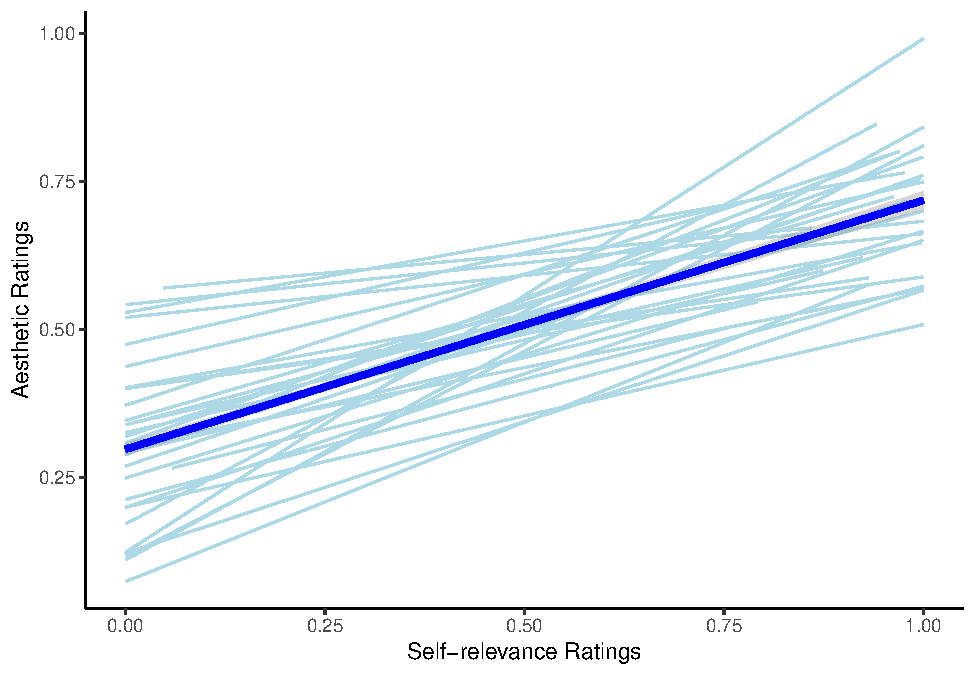
\includegraphics{11_files/figure-latex/unnamed-chunk-1-1.pdf}
\caption{\label{fig:unnamed-chunk-1}Exp 1A The association between aesthetic ratings and relevance}
\end{figure}

\hypertarget{experiment-1b}{%
\section{2.2 Experiment 1B}\label{experiment-1b}}

\hypertarget{participants-and-procedure-1}{%
\subsubsection{2.2.1 Participants and Procedure}\label{participants-and-procedure-1}}

A total of 208 participants were recruited and conducted online.

This experiment includes two blocks. In the first block, participants viewed each image for 5 s, followed by a screen on which they were required to rate each image on 10 different questions. A smaller version of the image was presented next to the rating scales. When all 10 questions had been answered, the participant clicked a ``next'' button to proceed to the next trial. For this experiment, we focused on two of these questions, which we refer to as ``beauty'' (``How much did you get the feeling of beauty?'') and ``being moved'' (``To what extent did the image move you?''). In the second block, participants saw each artwork again in a new random order and responded to the question, ``How self-relevant is the image to you?'' This single question and a continuous response scale were presented below the artwork, which remained on the screen until the participant used the mouse to answer and clicked ``next'' to proceed.

The answers regarding the ratings of beauty, being moved, and self-reference were subsequently recoded to values between 0 and 1. LMMs were computed to predict beauty and being moved ratings from self-relevance, using the same procedure and models as in Experiment 1A.

\hypertarget{results-1}{%
\subsubsection{2.2.2 Results}\label{results-1}}

Model comparison using AIC revealed that for beauty, Model 4 outperformed the others: log likelihood M1 = -283, M2 = -142, M3 = 1055, M4 = 1068, M4 versus M3, \emph{χ2} (2) = 25.0, \emph{p} \textless{} 4 ×10-6. For being moved, model 4 also performed best: log likelihood M1 = 627, M2 = 832, M3 = 1592, M4 = 1603, M4 versus M3, \emph{χ2} (2) = 22.5, \emph{p} \textless{} 1.3 ×10-5.
Individual ratings of self-relevance were again strongly predictive of aesthetic ratings of both beauty, slope = 0.31, 95\% CI = {[}0.28, 0.34{]}, \emph{t} (176.3) = 19.9, \emph{p} = 4.7 × 10-47, \emph{η²} = 0.69, and being moved, slope = 0.25, 95\% CI = {[}0.22, 0.28{]}, \emph{t} (154.5) = 15.2, \emph{p} = 1.4 × 10-32, \emph{η²} = 0.60 (\textbf{Figure 2 \& Figure 3}).

\begin{figure}
\centering
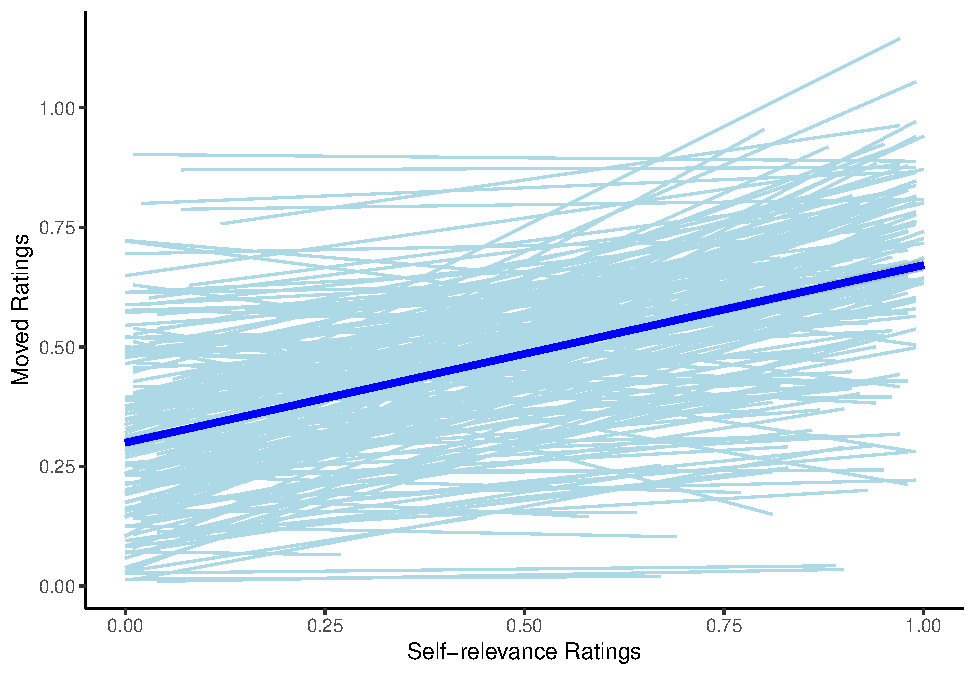
\includegraphics{11_files/figure-latex/unnamed-chunk-3-1.pdf}
\caption{\label{fig:unnamed-chunk-3}Exp 1B.The association between being moved ratings and relevance}
\end{figure}

\begin{figure}
\centering
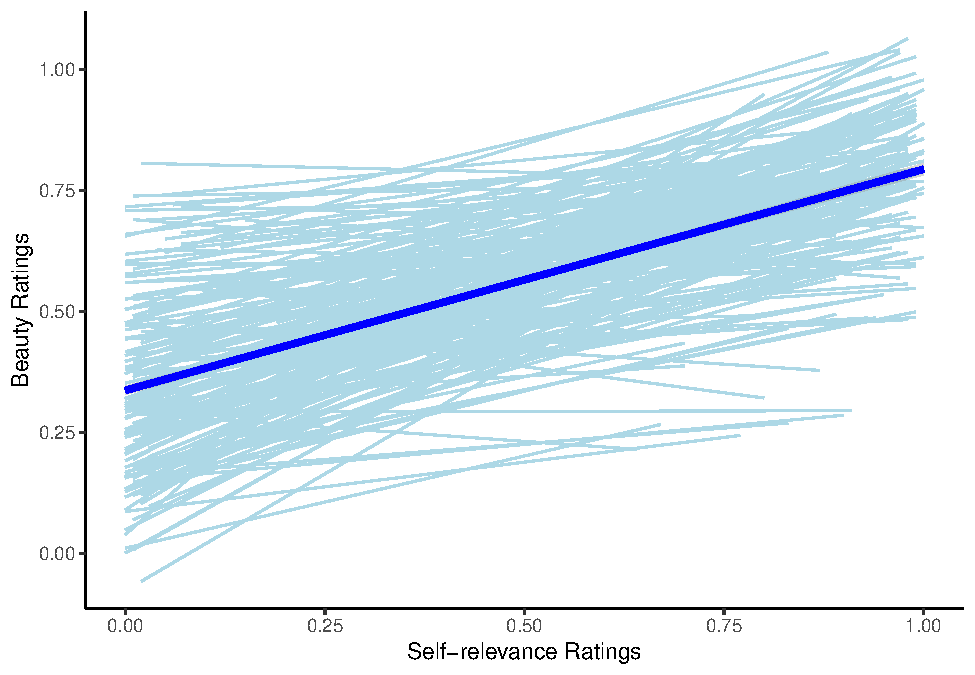
\includegraphics{11_files/figure-latex/unnamed-chunk-4-1.pdf}
\caption{\label{fig:unnamed-chunk-4}Exp 1B.The association between beauty ratings and relevance}
\end{figure}

\hypertarget{experiment-2}{%
\subsection{2.3 Experiment 2}\label{experiment-2}}

\hypertarget{participant-and-procedure}{%
\subsubsection{2.3.1 Participant and Procedure}\label{participant-and-procedure}}

A total of 59 participants were recruited online via Prolific, of which 45 (28 male, 15 females, age: M = 29.8 years, SD = 8.0) completed the experimental task. The stimulating materials include 80 artworks, with 20 in each of four conditions (self-relevant, other-relevant, generated-controland real artworks). Self-relevant artworks were generated using style transfer based on participants' responses to the Cultural Background and Lifestyle Questionnaire. Other-relevant artworks were generated for a matched participant, using the same styles but different content.

Generated-control artworks were generated using random content, but same styles as the self-relevant and other-relevant artworks. Real artworks were selected from a previous study, covering a variety of time periods, styles, genres, and cultural origins. The experiment consisted of two sessions. In session one, participants completed the Cultural Background and Lifestyle Questionnaire and were paired with a matched participant based on their responses.
In session 2, participants rated all 80 artworks for aesthetic appeal, self-relevance, and familiarity.

Artworks were presented in a pseudorandom order, with a fixation cross, the artwork, and a response screen.

Linear mixed models (LMM) were used to analyze the relationship between self-relevance and aesthetic appeal. Additional LMMs were used to compare the ratings of self-relevance and aesthetic appeal across the four conditions. A mediation analysis was conducted to investigate whether familiarity mediated the effect of self-relevance on aesthetic appeal. A regression analysis was performed to examine the relationship between aesthetic appeal and different aspects of self-relevance.

\hypertarget{results-2}{%
\subsubsection{2.3.2 Results}\label{results-2}}

Firstly, artworks from the self-relevant category were rated as significantly more self-relevant than all other categories (self-relevant vs.~other-relevant estimate = 0.19), 95\% CI = {[}0.16, 0.21{]}, \emph{d} = 0.59, \emph{t}(3160) = 13.0, \emph{p} = 1.3 ×10 -37. Real artworks were rated as less self-relevant than the generated-control artworks (real-artworks vs.~generated-control estimate = −0.031), 95\% CI = {[}--0.059, --0.003{]}, \emph{d} = −0.097, \emph{t}(3160) = −2.2, \emph{p} = .031. Other relevant artworks were also rated as more self-relevant than the generated-control artworks (other-relevant vs.~control-generated estimate = 0.064), 95\% CI = {[}0.036, 0.092{]}, \emph{d} = 0.20, \emph{t}(3160) = 4.5. Secondly, artworks generated from self-relevant content were rated as significantly more appealing than matched other-relevant artworks (self-relevant vs.~other-relevant estimate = 0.071), 95\% CI = {[}0.048, 0.095{]}, \emph{d} = 0.27, t(3160) = 5.9, \emph{p} = 3.8×10-9. Real artworks were rated as significantly more aesthetically appealing than the generated-control artworks (real artworks vs.~generated-control estimate = 0.046), 95\% CI = {[}0.023, 0.070{]}, \emph{d} = 0.17, \emph{t}(3160) = 3.8, \emph{p} = .00013, the self-relevant-generated artworks recovered this difference, even being slightly preferred to the real artworks on average (self-relevant vs.~real-artworks estimate = 0.014), 95\% CI = {[}--0.0097, 0.038{]}, \emph{d} = 0.052, \emph{t}(3160) = 1.2, \emph{p} = .25 (not significant). Lastly, a formal mediation analysis revealed that familiarity was able to explain only a small fraction of the self-relevance effect (Fig. 1e; average causal mediation effect = 0.04, 95\% CI = {[}0.03, 0.05{]}; remaining direct effect of self-relevance on aesthetic appeal = 0.33, 95\% CI = {[}0.30, 0.35{]}).

\begin{longtable}[]{@{}ccc@{}}
\caption{\label{tab:unnamed-chunk-5}Assessment of reproducibility}\tabularnewline
\toprule\noalign{}
RepeatabilityCondition & N & \% \\
\midrule\noalign{}
\endfirsthead
\toprule\noalign{}
RepeatabilityCondition & N & \% \\
\midrule\noalign{}
\endhead
\bottomrule\noalign{}
\endlastfoot
Totally Aligned(\texttt{δ} = 0\%) & 29 & 85.3 \\
Less Deviation(0\% \textless{} \texttt{δ} \textless{} 10\%) & 3 & 8.9 \\
Significant Deviation(\texttt{δ} \textgreater{} 10\%) & 2 & 5.9 \\
Deviation due to rounding & 0 & 0.0 \\
\end{longtable}

\hypertarget{discussion}{%
\section{3.Discussion}\label{discussion}}

In the present study, we explored the association between self-relevance and aesthetic appeal and examined the degree of reproducibility of this article. We found that aesthetic ratings of visual art are strongly correlated with self-relevance judgments (Experiments 1A and 1B), and individually customized synthetic artworks generated on the basis of participants' responses to a Cultural Background and Lifestyle Questionnaire were rated as more aesthetically appealing than either artworks generated for a different participant or a control set of artworks shown to all participants (Experiment 2). Furthermore, most of the experimental results have been accurately reproduced.

This study indicated that aesthetic ratings of visual art are strongly correlated with self-relevance judgments (Experiments 1A and 1B). It might due to the fact that high-order semantic and associative information generally matters more than low-level perceptual features for determining the aesthetic value that a person assigns to a visual image or experience.Addionally, information about the self resides at the top of that knowledge structure, that has encoding advantage. Given the centrality of the self-construct, it follows that acquiring information that relates to the self, and hence has the capacity to reduce uncertainty about central aspects of our world model, greater pleasure, and higher aesthetic valuation than a change in beliefs or resolution of ambiguity about a nonpersonal object or about a resolution of a perceptual ambiguity.

Experiment 2 manipulated self-relevance in artworks using style transfer and examined its impact on aesthetic appeal, self-relevant artworks are more appealing: Customized synthetic artworks generated based on participants' responses were rated as more aesthetically appealing than artworks generated for other individuals or a control set, demonstrating the significant influence of self-relevance on aesthetic judgments.Self-relevance is independent of image features and artistic skill: The effect of self-relevance on aesthetic appeal was not explained by intrinsic image properties or the artistic skill inherent in real artworks. This suggests that the connection between self and artwork is a distinct factor contributing to aesthetic value. Self-relevance is not mediated by familiarity: Although familiarity positively predicted aesthetic ratings, the effect of self-relevance on aesthetic appeal was not explained by familiarity.Self-relevant content increased appeal even when the content was not specifically rated as familiar.

The reproduction of most of the data indicates that we successfully replicated the main results and trends in the experiment, suggesting that the original study's findings are robust and reproducible. However, we also observed discrepancies between a small fraction of the data and the results reported in the original study. Specifically, the results in experiment 1B found that there was a slight deviation in the p-values for model comparisons; and in experiment 2, there were three p value and a t value deviated from the results reported in the literature. These differences may arise from a variety of factors. Firstly, there might have been an error in the data recording process. Besides, differences in software versions and environment settings can also lead to slight deviations in the calculation results. Additionally, the duplicator has a vulnerability in their knowledge or operation of R.

\textbf{Authors' contribution:}
Qiu Zhipeng (Group leader):Responsible for overall coordination, code analysis(25\%),and PPT presentation;
Wu Yuxin:Responsible for code analysis(25\%), PPT production(33\%), and report writing for experiment 1A;
Ni Fengmin:(Responsible for code analysis(25\%), PPT production (33\%), and report writing for experiment for experiment 1B and the introduction and the code structure introduction;
Han Yi:Responsible for code analysis (25\%), PPT production (33\%), and report writing for experiment 2.

\hypertarget{reference}{%
\section*{Reference}\label{reference}}
\addcontentsline{toc}{section}{Reference}

\hypertarget{refs}{}
\begin{CSLReferences}{1}{0}
\leavevmode\vadjust pre{\hypertarget{ref-andrews-hanna_functional-anatomic_2010}{}}%
Andrews-Hanna, J. R., Reidler, J. S., Sepulcre, J., Poulin, R., \& Buckner, R. L. (2010). Functional-anatomic fractionation of the brain's default network. \emph{Neuron}, \emph{65}(4), 550--562. \url{https://doi.org/10.1016/j.neuron.2010.02.005}

\leavevmode\vadjust pre{\hypertarget{ref-dargembeau_neural_2010}{}}%
D'Argembeau, A., Stawarczyk, D., Majerus, S., Collette, F., Van der Linden, M., Feyers, D., \ldots{} Salmon, E. (2010). The neural basis of personal goal processing when envisioning future events. \emph{Journal of Cognitive Neuroscience}, \emph{22}(8), 1701--1713. \url{https://doi.org/10.1162/jocn.2009.21314}

\leavevmode\vadjust pre{\hypertarget{ref-leder_private_2016}{}}%
Leder, H., Goller, J., Rigotti, T., \& Forster, M. (2016). Private and {Shared} {Taste} in {Art} and {Face} {Appreciation}. \emph{Frontiers in Human Neuroscience}, \emph{10}. \url{https://doi.org/10.3389/fnhum.2016.00155}

\leavevmode\vadjust pre{\hypertarget{ref-menninghaus_distancing-embracing_2017}{}}%
Menninghaus, W., Wagner, V., Hanich, J., Wassiliwizky, E., Jacobsen, T., \& Koelsch, S. (2017). The {Distancing}-{Embracing} model of the enjoyment of negative emotions in art reception. \emph{Behavioral and Brain Sciences}, \emph{40}, e347. \url{https://doi.org/10.1017/S0140525X17000309}

\leavevmode\vadjust pre{\hypertarget{ref-pelowski_move_2017}{}}%
Pelowski, M., Markey, P. S., Forster, M., Gerger, G., \& Leder, H. (2017). Move me, astonish me\ldots{} delight my eyes and brain: {The} {Vienna} {Integrated} {Model} of top-down and bottom-up processes in {Art} {Perception} ({VIMAP}) and corresponding affective, evaluative, and neurophysiological correlates. \emph{Physics of Life Reviews}, \emph{21}, 80--125. \url{https://doi.org/10.1016/j.plrev.2017.02.003}

\leavevmode\vadjust pre{\hypertarget{ref-talarico_emotional_2004}{}}%
Talarico, J. M., LaBar, K. S., \& Rubin, D. C. (2004). Emotional intensity predicts autobiographical memory experience. \emph{Memory \& Cognition}, \emph{32}(7), 1118--1132. \url{https://doi.org/10.3758/bf03196886}

\leavevmode\vadjust pre{\hypertarget{ref-vessel_stronger_2018}{}}%
Vessel, E. A., Maurer, N., Denker, A. H., \& Starr, G. G. (2018). Stronger shared taste for natural aesthetic domains than for artifacts of human culture. \emph{Cognition}, \emph{179}, 121--131. \url{https://doi.org/10.1016/j.cognition.2018.06.009}

\leavevmode\vadjust pre{\hypertarget{ref-wagner_representation_2012}{}}%
Wagner, D. D., Haxby, J. V., \& Heatherton, T. F. (2012). The {Representation} of {Self} and {Person} {Knowledge} in the {Medial} {Prefrontal} {Cortex}. \emph{Wiley Interdisciplinary Reviews. Cognitive Science}, \emph{3}(4), 451--470. \url{https://doi.org/10.1002/wcs.1183}

\end{CSLReferences}


\end{document}
